% 第1章 索洛模型与序列视角下的动态优化

% 导言

\chapter{序列视角下的动态优化} \label{ch-dynamic-opt-sq}

现代宏观经济学通过优化经济主体行为来研究经济运行的动态运行过程。因此，动态优化是学习量化宏观的基础。
宏观经济理论发展至今，对动态优化问题形成了两种处理方法：
一是序列问题视角，通过求解差分（微分）方程为经济主体选择一个最优的序列（有限或是无穷），这是处理动态问题的基础视角；
二是递归视角：定义从当期到下期的映射，利用动态规划方法将优化问题转化为泛函方程的求解。

本章通过宏观经济学中两种重要模型对序列视角下的动态优化进行初步介绍：消费-储蓄模型和新古典增长模型。
借助消费-储蓄问题，我们将初步了解优化问题的序列求解方法。
接着，我们将详细学习新古典增长理论：先对经典的索洛模型进行回顾，深化对动态宏观基本概念和理论的认识；
然后，借助现代宏观经济学的基石模型（Workhouse Model）——新古典增长模型（或称最优增长模型），
深化对序列视角下动态优化理论的理解，为下一章递归方法和动态规划学习奠定基础。


% =============== main ch1 ===============

% 1.1 =============== 消费-储蓄模型 ===============

\section{动态优化引例：消费-储蓄问题} \label{sec-consumption-saving}



% 1.2 =============== 新古典理论 ===============

\section{新古典增长理论} \label{sec-ngm}

接下来，我们将通过另一个重要模型来深入对序列视角下动态优化问题的认知，这就是新古典增长模型（或称最优增长模型）。
新古典理论是在Solow等人的工作之上建立起来的。在当时，美国长期稳定的资本产出比引起了许多经济学家的关注。
早期增长理论如哈罗德-多马模型将这一特征直接作为模型的前提假设：资本与劳动必须按固定比例结合（互补）才能进行生产。
但是索罗发现，资本和劳动明显是可替代的，传统理论不能解释现实问题：
数据上看，劳动的价格（工资）趋势性上升，在生产要素互补的情形下，资本租金率也应当上升，这与观察到的稳定的资本租金率不符。

索洛认为，这些现象可以由\textbf{新古典}视角加以解释。如果一个生产函数关于其投入要素是\textbf{边际报酬递减的}，
我们通常称其具有\textbf{新古典特征}。在这一生产函数下，当人均资本提高，资本的边际产出会降低，在竞争市场上这会反应为要素价格的变化。
而如果同时存在劳动增进的技术进步，就可以解释特征事实中要素数量和价格的相关特征。由此，一个将新古典特征和技术进步相结合的理论诞生了。
Solow（1956）和Swan（1956）在Ramsey（1928）、哈罗德-多马模型等理论的基础上，建立了Solow-Swan模型，
奠定了新古典增长理论（Neoclassical Growth）和现代宏观经济学的基础。

在本节我们将重点介绍新古典增长模型的起源——索洛模型，并引出相关宏观经济学的概念。
我们将在下一节重点研究最优增长模型的序列化解法。


% 1.2.1 ===== 基准 =====
\subsection{基准索洛模型}

索洛模型的核心要素是\textbf{总量生产函数}（Aggregate Production Function），
通常由总资本$K_t$，总劳动投入$L_t$（人口乘人均工作时间）和技术$A_t$构成。
我们从最简单的情形开始来介绍相关概念。在这一模型中，没有技术进步或人口和工人技能特征，从而总量生产函数为：
\begin{equation*}
    Y_t = F\left(K_t, L_t\right)
\end{equation*}
其中$Y_t$可以理解为经济的GDP。对于函数$F(K, L)$，有如下假设：
\begin{assumption}  \label{as-F-increase}
    $F(K, L)$关于$k$和$L$严格递增
\end{assumption}
\begin{assumption}  \label{as-F-quasiconcave}
    $F(K, L)$关于$(K, L)$严格拟凹
\end{assumption}
\begin{assumption}  \label{as-F-cosntant}
    $F(K, L)$关于$(K, L)$规模报酬不变
\end{assumption}
\begin{assumption}  \label{as-F-zero}
    $F(0, L)=0$
\end{assumption}
\begin{assumption}  \label{as-F-inada}
    \textbf{Inada条件}：$\lim\limits_{K\rightarrow 0}F_1(K, L)
        = \infty, \quad \lim\limits_{K\rightarrow \infty}F_1(K, L)=0$
\end{assumption}

在基准模型中，假设人口总数$N_t$和人均工作时间$l_t$为常数，因此$L_t$为常数。
将人口总数和人均工时正则化为1，从而生产函数中剩下的变量只有$K_t$，结合规模报酬不变，可以写出人均形式：
\begin{equation*}
    F(K_t, 1)=F(k_t, 1)\equiv f(k_t)
\end{equation*}
我们以小写字母表示人均测度，生产函数可以表示为：
\begin{equation}
    y_t = f(k_t)
\end{equation}
索洛模型的另一个核心构成是\textbf{资本运动方程}：
\begin{equation}    
    k_{t+1} = i_t + (1-\delta)k_t
\end{equation}
其中$i_t$表示$t$期的（人均）投资，$\delta k_t$表示既有资本的折旧，$\delta\in (0,1)$表示折旧率。
索洛模型隐性地假定了产品的同质性，可被用于消费或投资,根据供给等于需求：
\begin{equation}
    y_t = c_t + i_t
\end{equation}
在索洛模型中，并没有对消费者的消费-储蓄问题建模，而是假设\textbf{外生储蓄率}$s\in(0,1)$。
由于$y_t$不仅是产品供给，同时也是消费者的总收入，即它不是被用于消费就是被用于储蓄，因此总投资等于总储蓄：
\begin{equation}
    i_t = s y_t
\end{equation}
从而我们可以得到\textbf{资本运动方程的差分形式}：
\begin{equation}    \label{eq-k-law-of-motion}
    k_{t+1} = (1-\delta)k_t + sf(k_t)
\end{equation}
这是索洛模型的核心方程：右侧唯一的内生变量是资本存量$k_t$，下期的内生资本水平仅由当期资本水平决定。
注意到，对于外生给定的$k_0$，我们可以由上式得到资本序列$\{k_{t+1}\}_{t=0}^{\infty}$，
进而同时也能得到人均产出、消费和投资（储蓄）。


% 1.2.2 ===== 稳态 =====
\subsection{稳态与动态}

对\cref{eq-k-law-of-motion}，考虑$k_t$不随时间变化这一特殊情形，我们称其为\textbf{稳态}，
记为$k_t=\bar{k},~\forall t$。它是如下方程的解：
\begin{equation*}
    \bar{k}=(1-\delta) \bar{k}+s f(\bar{k})
\end{equation*}
这表明在稳态时，$\delta \bar{k} = sf(\bar{k})$。方程左侧是一条通过原点的直线；
方程右侧是通过原点、严格递增并且严格凹的曲线，它在0处斜率趋近无穷，$\bar{k}\rightarrow \infty$时斜率趋近0。
这样的\textbf{Inada条件}保证了严格正的解$\bar{k}$存在且唯一。不难看出，Inada条件是一个充分条件，它可以减弱为：
$\lim\limits_{k\rightarrow 0}F_1(k,1)>\delta/s$和$\lim\limits_{k\rightarrow \infty}F_1(k,1)<\delta/s$。
同时，在稳态下，$k_t/y_t$为常数，这与特征事实相符。假设柯布-道格拉斯生产函数的话，稳态时资本产出比为：
\begin{equation*}
    \frac{\bar{k}}{\bar{y}} = \frac{s}{\delta}
\end{equation*}

接下来，我们利用\textbf{相图}（Diagram）分析当初始$k_0>0$不处于稳态值时，$k_t$的\textbf{动态}。
\cref{dynamics-solow}绘制了资本运动方程\cref{eq-k-law-of-motion}和45度线，其中横轴是当期资本，纵轴是下期资本，
因此45度线代表资本处于稳态。给定横轴上一个初始$k_0$，由\cref{eq-k-law-of-motion}可以在纵轴上得到下期的$k_1$；
再将$k_1$做为新的初始状态，利用\cref{eq-k-law-of-motion}在纵轴上得到$k_2$，依次进行下去，
可以得到资本序列$\{k_{t+1}\}_{t=0}^{\infty}$。显然，只要初始$k_0>0$，无论从何处开始，系统最终都会收敛至稳态$\bar{k}$。
更严谨的论证如下：假设$k_t<\bar{k}$，从而有$sf(k_t)>\delta k_t$，进而$k_{t+1}>k_t$。
同时，由于$k_t<\bar{k}$，因此$k_{t+1}=(1-\delta)k_t+sf(k_t)<(1-\delta)\bar{k}+sf(\bar{k})=\bar{k}$。
重复上述程序，可以得到一个\textbf{单调有界序列}$\{k_t,k_{t+1},k_{t+1},\cdots\}$，其界为$\left[k_t,\bar{k}\right]$。
由单调收敛定理可知这一序列存在极限，并且根据给定的条件，极限唯一，因此必为$\bar{k}$。同理可证$k_t>\bar{k}$的情形。

\begin{figure}
    \centering
    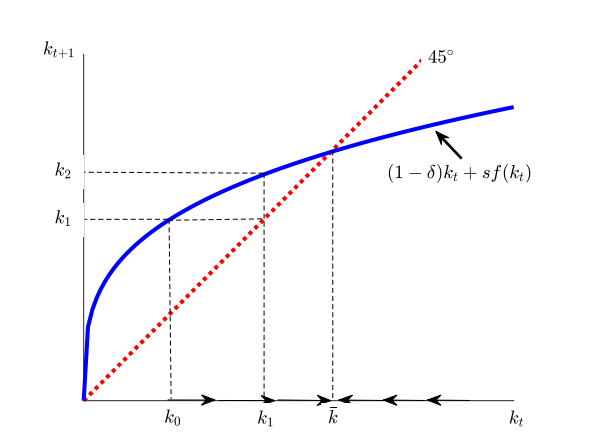
\includegraphics[width=0.8\textwidth]{figures/part1/ch1/dynamics-solow.png}
    \caption{索洛模型的动态}
    \label{dynamics-solow}
\end{figure}

直觉上讲，收敛的原因在于生产函数关于资本的边际报酬递减（\cref{as-F-quasiconcave}）。根据资本运动方程：
\begin{equation*}
    k_{t+1}-k_{t} = i_t - \delta k_t
\end{equation*}
有两种相反力量影响资本的运动：总投资和折旧。给定外生储蓄率，当资本存量较低时，单位资本的产出较高，
$i_t=sf(k_t)$相对于折旧的资本更高，从而资本存量逐渐提高。但在这一过程中，由于资本边际报酬递减，单位资本的产出逐渐降低，
当$k_t$足够大时，对应资本存量下的总投资不再能覆盖折旧，资本存量最终达到稳态。
进一步将资本运动方程变换为增长率形式：
\begin{equation*}
    \frac{k_{t+1}-k_t}{k_t} = \frac{s f\left(k_t\right)}{k_t}-\delta
\end{equation*}
根据$f^{\prime\prime}(k_t)<0$和$f(0)=0$的假设，$f(k_t)/k_t$关于$k_t$递减，这带来了投资对于资本存量的推动和
折旧随资本存量水平提高而增加这两种相反力量。


% 1.2.3 ===== Balanced Growth =====
\subsection{技术进步与平衡增长路径}

在基础模型中，我们省去了技术进步$A_t$和劳动投入$L_t$，经济在长期达到恒定稳态。在本节，我们引入两个新的特征：
一是允许劳动投入$L_t$（人口乘人均工时）随时间增长；二是引入技术进步$A_t$。从而生产函数形式为：
\begin{equation*}
    Y_t = F\left(K_t, A_tL_t\right)
\end{equation*}
也就是说，技术进步表现为劳动投入的改善。$A_tL_t$通常被称为\textbf{有效劳动}（Efficiency Labor）；
这一形式的技术进步被称为\textbf{劳动增广型}或\textbf{哈罗德中性}（Harrod-Neutral）。
\footnote{事实上，劳动增广型技术进步是唯一与平衡增长相合的技术进步形式（即所有总量变量以相同速率增长）。}
假设技术$A_t$的进步率为$\gamma$，劳动投入$L_t$的增长率为$n$。
\footnote{$n$可能有两个来源：一是人口的变化；二是人均工时的变化。}
总量形式的资本运动方程为：
\begin{equation*}
    K_{t+1}=(1-\delta) K_t+s F\left(K_t, A_t L_t\right)
\end{equation*}
由于技术进步的存在，显然是不存在上面所看到的严格意义的稳态的。
不过，通过正则化相关变量，我们能够将其转化为\textbf{平稳的变量}。两边同时除以有效劳动$A_tL_t$：
\begin{equation*}
    \frac{K_{t+1}}{A_t L_t}=(1-\delta) \frac{K_t}{A_t L_t}+s \frac{F\left(K_t, A_t L_t\right)}{A_t L_t}
\end{equation*}
通常称这一正则化后的变量为有效人均劳动，记为：
\begin{equation*}
    \tilde{k}_t \equiv \frac{K_t}{A_tL_t}
\end{equation*}
从而资本运动方程可以改写为\textbf{有效人均形式}：
\begin{equation*}
    \frac{A_{t+1}}{A_t} \frac{L_{t+1}}{L_t} \frac{K_{t+1}}{A_{t+1} L_{t+1}}=(1-\delta) 
        \frac{K_t}{A_t L_t}+s F\left(\frac{K_t}{A_t L_t}, 1\right)
\end{equation*}
即：
\begin{equation}    \label{eq-k-law-of-motion-bgp}
    (1+\gamma)(1+n) \tilde{k}_{t+1}=(1-\delta) \tilde{k}_t+s f(\tilde{k}_t)
\end{equation}
其中，$f(\tilde{k}_t) \equiv F(\tilde{k}_t,1)$。
对正则化后的资本和上述运动方程，可以得到稳定的稳态值，进而可以再将其转化为宏观变量。

事实上，对应于基准模型下的稳态，我们使用\textbf{平衡增长路径}（Balanced Growth Path）来刻画这类带有增长特征模型的长期行为。
\footnote{部分学者仍使用稳态来表示平衡增长路径，因为正则化后的变量具有严格稳定的稳态值。}
在平衡增长路径下，$\tilde{k}_t$是常数，宏观变量如$Y_t,~K_t,~C_t$\textbf{以相同的常速率增长}。
将平衡增长路径下的有效人均资本记为：$\tilde{k}_{t+1}=\tilde{k}_t=\bar{\tilde{k}}$，它是如下方程的解：
\begin{equation*}
    (1+\gamma)(1+n) \overline{\tilde{k}}=(1-\delta) \overline{\tilde{k}}+s f(\overline{\tilde{k}})
\end{equation*}
对于转换后的平稳变量，其动态特征与基准模型相近：从任意$\tilde{k}_0$开始，$\{\tilde{k}_{t+1}\}_{t=0}^{\infty}$
单调收敛到$\bar{\tilde{k}}$。

进一步分析哈罗德中性模型中经济变量的特征。假设所有劳动力都工作1单位，即$L_t$只表示总人口，
人均产出定义为$y_t\equiv Y_t/L_t$。由于在长期$Y_t /\left(A_t L_t\right)=f(\tilde{k}_t)$
收敛到$f(\bar{\tilde{k}})$，因此人均资本收敛到：
\begin{equation*}
    y_t = f(\bar{\tilde{k}})A_t
\end{equation*}
在长期，人均产出的增长率为：
\begin{equation*}
    \frac{y_{t+1}-y_t}{y_t}=\frac{f(\bar{\tilde{k}}) A_{t+1}-f(\bar{\tilde{k}}) A_t}{f(\bar{\tilde{k}}) A_t}
        =\frac{A_{t+1}-A_t}{A_t}=\gamma
\end{equation*}
也就是说，在平衡增长路径上，人均产出以$\gamma$的速率增长，其余参数如储蓄率$s$不会影响\textbf{长期速率}。

需要注意的是，上述结果说外生储蓄率对经济没有影响：它会影响人均产出的\textbf{水平值}。
同时，当经济尚未收敛到平衡增长路径上时，外生储蓄率的水平也会影响经济短期的增长率，因为短期内$\tilde{k}_t$的变动会产生影响：
\begin{equation*}
    \frac{y_{t+1}-y_t}{y_t} = 
        \frac{f(\tilde{k}_{t+1}) A_{t+1}-f(\tilde{k}_t) A_t}{f(\tilde{k}_t) A_t} = 
            \frac{f(\tilde{k}_{t+1})}{f(\tilde{k}_t)}(1+\gamma)-1
\end{equation*}
根据有效人均形势下的资本运动方程\cref{eq-k-law-of-motion-bgp}：当$\tilde{k}_t<\bar{\tilde{k}}_t$，$\tilde{k}_t$随时间增长，
即$\tilde{k}_{t+1}>\tilde{k}_t$。此时$f(\tilde{k}_{t+1})/f(\tilde{k}_t)>1$，短期内人均产出增长率高于$\gamma$。
同理，当$\tilde{k}_t>\bar{\tilde{k}}_t$，短期内人均产出增长率小于$\gamma$。


% 1.2.4 ===== 特征事实 ====
\subsection{特征事实：数据与模型}

回顾索洛模型的动机之一：解释资本产出比的长期稳定性。在长期平衡增长路径下，$Y_t/(A_tL_t) = f(\tilde{k}_t)$
和$K_t/(A_tL_t)=\tilde{k}_t$都是常数，从而$K_t/Y_t=\tilde{k}_tf(\tilde{k}_t)$也是常数。
因此索洛模型可以解释稳定的资本产出比这一特征事实。同时，在平衡增长路径下，人均产出增速稳定为$\gamma$，
这也与特征事实相匹配。

另外一层特征事实是要素价格方面的：物质资本回报率几乎稳定。我们首先需要在模型中对其进行计算。
假设厂商在竞争市场上最大化其利润：
\begin{equation}
    \max _{K_t, A_t L_t} F\left(K_t, A_t L_t\right)-r_t K_t-w_t A_t L_t
\end{equation}
简单起见，假设消费者拥有资本并将其出售给厂商，即$r_t$代表资本回报率。根据一阶条件：\textbf{资本回报率等于资本的边际产出}，即：
\begin{equation*}
    r_t = F_1\left(K_t, A_tL_t\right) 
\end{equation*}
对$f(K_t/A_tL_t) \equiv F\left(K_t, A_tL_t\right)/(A_tL_t)$两侧同时对$K_t$微分
可知：$\frac{f^{\prime}(\tilde{k}_t)}{A_tL_t}=\frac{F_1\left(K_t, A_tL_t\right)}{A_tL_t}$，从而成立：
\begin{equation*}
    r_t = f^{\prime}(\tilde{k}_t)
\end{equation*}
在长期平衡增长路径下，$\tilde{k}_t$为常数，$f^{\prime}(\tilde{k}_t)$为常数，$r_t$也为常数，与特征事实相符。

此外，当时美国经济的另一特征事实在于劳动和资本份额的稳定性。在模型中，资本份额可以表示为$r_tK_t/Y_t$，
由于我们已经证明了$K_t/Y_t$和$r_t$在长期平衡增长路径下都是稳定的，因此模型中资本份额的长期特征也能与特征事实相匹配。
对于劳动份额，在模型中可以表示为$w_tA_tL_t/Y_t$。由厂商问题的一阶条件：
\begin{equation*}
    w_t = F_2\left(K_t, A_tL_t\right)
\end{equation*}
同时，对于规模报酬不变的生产函数，它是一次齐次的，即：
\begin{equation*}
    qF\left(K_t,A_tL_t\right) = F\left(qK_t,qA_tL_t\right)
\end{equation*}
两边同时对$q$微分：
\begin{equation*}
    F\left(K_t,A_tL_t\right) = K_tF_1\left(qK_t,qA_tL_t\right) + A_tL_tF_2\left(qK_t,qA_tL_t\right)
\end{equation*}
由于上式恒成立，因此在$q=1$处有：
\begin{equation*}
    Y_t = F\left(K_t,A_tL_t\right) = K_tF_1\left(K_t,A_tL_t\right) + A_tL_tF_2\left(K_t,A_tL_t\right)
\end{equation*}
结合劳动的一阶条件，并将两边同时除以$Y_t$，可知劳动份额等于1减去资本份额：
\begin{equation*}
    w_tA_tL_t/Y_t = 1 - r_tK_t/Y_t
\end{equation*}
实际上，与证明资本份额类似，通过直接计算的方式也可以得到模型中劳动份额的特征。
对$f(K_t/A_tL_t) \equiv F\left(K_t, A_tL_t\right)/(A_tL_t)$两侧同时对$A_tL_t$微分可知：
\begin{equation*}
    -\frac{f^{\prime}(\tilde{k}_t)K_t}{(A_tL_t)^2} 
        = \frac{F_2(K_t,A_tL_t)A_tL_t - F\left(K_t, A_tL_t\right)}{(A_tL_t)^2}
\end{equation*}
结合一阶条件可得：
\begin{equation*}
    w_t = f(\tilde{k}_t) - \tilde{k}_tf^{\prime}(\tilde{k}_t)
\end{equation*}
在平衡增长路径下$\tilde{k}_t=\bar{\tilde{k}}$，工资为常数，从而资本份额$w_tA_tL_t/Y_t=w_t/f(\tilde{k}_t)$为常数，
与特征事实相符。特别的，对柯布-道格拉斯生产函数$Y_t=K_t^{\alpha}(A_tL_t)^{1-\alpha}$，即使在平衡增长路径外，
资本和劳动份额始终恒定为$\alpha$和$1-\alpha$。


% 1.2.5 ===== 收敛性分析 ===== 
\subsection{收敛性分析}

我们已经看到，在索洛模型中，经济会单调收敛至稳态或平衡增长路径。在本小节，我们对收敛性进行一些更详细的说明。
回忆最简单的基准情形，我们将劳动投入$L_t$正则化为1，以人均形式描述经济过程。
由一阶泰勒展开，资本运动方程\cref{eq-k-law-of-motion}在\textbf{稳态附近}可以进行如下估计：
\begin{equation}
    \Delta k_{t+1}=\left(1-\delta+s f^{\prime}(\bar{k})\right) \Delta k_t
\end{equation}
其中$\Delta k_{t}$表示$k_t$对其稳态值的偏离（当偏离很小时），即$k_t-\bar{k}$。两边同除以$\bar{k}$得到：
\begin{equation}
    \frac{k_{t+1}-\bar{k}}{\bar{k}}=(1-\lambda) \frac{k_t-\bar{k}}{\bar{k}}
\end{equation}
其中，$\lambda = \delta - sf^{\prime}(\bar{k})$表示\textbf{收敛速度}。
$\lambda$越大，$\Delta k_{t+1}$缩小（绝对值）得更快，即系统向稳态收敛速度快。
如\cref{fig-convergence-speed}所给出的，$\lambda$越大，资本运动方程在稳态附近斜率更平，更快到达稳态。
假设柯布-道格拉斯生产函数，一阶展开可写为：
\begin{equation}
    \Delta k_{t+1}=\left(1-\delta(1-\alpha)\right) \Delta k_t
\end{equation}
收敛速度方程为：
\begin{equation}
    \lambda = \delta(1-\alpha)
\end{equation}
因此，资本份额$\alpha$越低、折旧率$\delta$越大，则收敛速度越快。

\begin{figure}
    \centering
    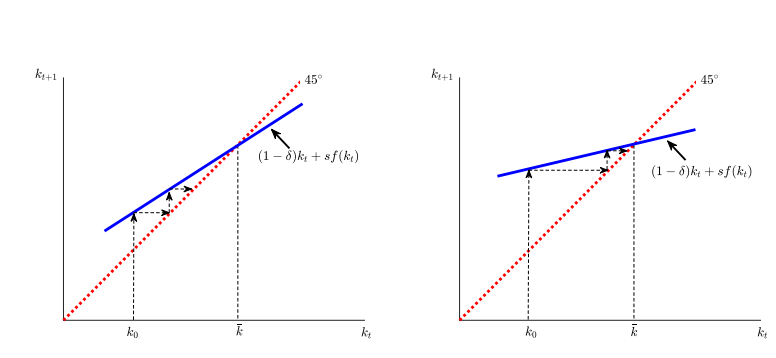
\includegraphics[width=1\textwidth]{figures/part1/ch1/convergence-speed.png}
    \caption{收敛速度}
    \label{fig-convergence-speed}
\end{figure}

一般而言，$k_t$如何影响$k_{t+1}$决定了收敛速度。例如，若$k_t$对$k_{t+1}$无影响，那么收敛会立刻实现，
即在\cref{fig-convergence-speed}反应为水平的直线。
不难看出，外生储蓄率$s$在柯布-道格拉斯生产函数下不会影响收敛速度，这是两个相反力量所导致的：
对给定的一个$k_t$，高的储蓄率$s$意味着$k_t$对$k_{t+1}$的影响更大；但更高的储蓄率也带来更高的稳态$\bar{k}$，
进而稳态时资本的边际产出$f^{\prime}(\bar{k})$低，这意味着$k_t$对$k_{t+1}$的影响更小。
在CD生产函数下，这两种作用相互抵消。

进一步回忆带有增长特征的索洛模型：
对其有效人均形式的资本运动方程\cref{eq-k-law-of-motion-bgp}在稳态附近进行一阶泰勒展开可得：
\begin{equation}
    (1+\gamma)(1+n) \Delta \tilde{k}_{t+1}
        = \left(1-\delta+s f^{\prime}(\overline{\tilde{k}})\right) \Delta \tilde{k}_t
\end{equation}
两边同时除以$\bar{\tilde{k}}$，得到收敛速度方程：
\begin{equation*}
    \frac{\tilde{k}_{t+1}-\bar{\tilde{k}}}{\tilde{\tilde{k}}}
        = (1-\lambda) \frac{\tilde{k}_t-\bar{\tilde{k}}}{\tilde{\tilde{k}}}
\end{equation*}
其中收敛速度为：
\begin{equation*}
    \lambda=1-\frac{1-\delta+s f^{\prime}(\bar{\tilde{k}})}{(1+\gamma)(1+n)} 
\end{equation*}
类似的，在柯布-道格拉斯生产函数下，一阶展开可写为：
\begin{equation*}
    \Delta \tilde{k}_{t+1}
        = \left(\alpha+\frac{(1-\alpha)(1-\delta)}{(1+\gamma)(1+n)}\right) \Delta \tilde{k}_t
\end{equation*}
收敛速度为：
\begin{equation*}
    \lambda = (1-\alpha)\left(1-\frac{1-\delta}{(1+\gamma)(1+n)}\right)
\end{equation*}


% 1.2.6 ===== 增长核算 ===== 
\subsection{应用索洛模型：增长核算}

更一般化的，Solow（1957）提出增长核算（Growth Accounting）的概念，用于研究不同生产要素对经济增长的作用。假设如下：
\begin{assumption}
    总产出$Y_t$由总量生产函数$F_t\left(K_t,L_t\right)$决定，$F$的时间记号保留了技术进步促进生产函数向上移动的可能；
\end{assumption}
\begin{assumption}
    $F$规模报酬不变及其余新古典性质；
\end{assumption}
\begin{assumption}
    投入要素完全竞争，即厂商最大化其利润。
\end{assumption}

微观经济学证明了，在完全竞争均衡情形下，规模报酬不变最终带来\textbf{零利润}，这也是索洛增长核算的起点。
与前面的记号类似，以小写字母表示人均测度，假设人口总量为$N_t$，根据规模报酬不变，我们可以将\textbf{人均产出}
表示为$y_t=F_t\left(k_t,l_t\right)$，其中$k_t\equiv K_t/N_t$和$l_t\equiv L_t/N_t$表示人均资本和人均工作时间。
假设人口总量不变，并将其正则化为1，可以得到$y_t=Y_t$。
\footnote{在基准模型中，我们额外假设了人均工时为常数，进而将其也正则化为1，因此基准模型是没有考虑劳动的。}
对此处的人均产出进行全微分可得：
\begin{equation}
    \begin{aligned}
        dy &= \frac{\partial F}{\partial t}dt + \frac{\partial F}{\partial k}dk + \frac{\partial F}{\partial l} \\
            &=  \frac{\partial F}{\partial t}dt 
                + \frac{\partial F}{\partial k} k \frac{dk}{k} + \frac{\partial F}{\partial l} l \frac{dl}{l}
    \end{aligned}
\end{equation}
其中所有的全微分都在$\left(t,k_t,l_t\right)$处取得。
在此处，为了方便取导数，我们假设了时间连续，但离散情形下并没有本质区别，只是记号的差异。
记$r_t, w_t$为完全竞争市场上的资本租金率和工资，厂商最大化利润问题为：
\begin{equation*}
    \max _{k, \ell} F_t(k, \ell)-r k-w l
\end{equation*}
根据一阶条件可得：
\begin{align}
    r &= \partial F / \partial k \\
    w &= \partial F / \partial l
\end{align}
两边同时除以总产出可得：
\begin{equation}
    \frac{d y}{y} = \frac{\partial F}{\partial t} 
        \frac{d t}{y} + \frac{r k}{y} \frac{d k}{k} + \frac{w l}{y} \frac{d l}{l}
\end{equation}
假设$1-\alpha$为劳动收入份额（可能时变，根据数据可计算），那么由规模报酬不变的零利润条件可知：资本份额为$\alpha$，
从而得得如下\textbf{增长核算方程}：
\begin{equation}
    \frac{d y}{y}=\frac{\partial F}{\partial t} \frac{d t}{F}+\alpha \frac{d k}{k}+(1-\alpha) \frac{d l}{l}
\end{equation}
其中，$\frac{\partial F}{\partial t}\frac{dt}{F}$被称为\textbf{索洛剩余}（Solow Residual），
因为它是不能由资本和劳动增长核算得到的部分，但可以通过作差得到，它测度了生产可能前沿如何随时间变动。

上述形式是一般化地将时间对生产函数的影响进行表示。我们可能对以下形式更为熟悉：
$F_t\left(k_t, l_t\right) \equiv A_tF\left(k_t, l_t\right)$，
由于$F$为一次齐次，因此这一形式被称为\textbf{希克斯中性}（Hicks-Neutral），
$A$被称为\textbf{全要素生产率}（Total Factor Productivity，TFP）。
$F\left(k_t,l_t\right)$是时间独立的函数，通过全微分可得到核算方程为：
\begin{equation}
    \frac{d y}{y}=\frac{d A}{A}+\alpha \frac{d k}{k}+(1-\alpha) \frac{d l}{l}
\end{equation}
若生产函数形式是\textbf{哈罗德中性}：$F_t\left(k_t, l_t\right) = F\left(k_t, A_tl_t\right)$，
此时$F$也是时间独立的，由厂商一阶条件$\frac{\partial F}{\partial l}=w/A$以及$wl=(1-\alpha)F$，
可类似的得到增长核算方程：
\begin{equation}
    \frac{d y}{y}=(1-\alpha) \frac{d A}{A}+\alpha \frac{d k}{k}+(1-\alpha) \frac{d l}{l}
\end{equation}

% 1.3 =============== 最优增长模型 ===============

\section{最优增长：RCK模型} \label{sec-opt-growth}

Solow（1956）和Swan（1956）的工作标志新古典增长理论的诞生。但Solow模型的主要问题在于，模型中储蓄率是外生给定的。
Cass（1965）和Koopmans（1965）在Solow工作的基础上，通过引入微观基础对新古典理论进行了拓展，
建立了确定性情形下的\textbf{最优增长模型}：他们利用家庭偏好来解释为何储蓄是一种内生理性选择的结果。
最优增长模型通常被称为RCK模型（Ramsey-Cass-Koopmans Model），它与消费-储蓄模型的核心区别在于：经济是生产经济而不是禀赋经济。
我们将利用这一模型，深入研究序列视角下的动态优化问题。

典型的确定性最优增长模型形式如下：假设时间是离散且无穷的，由$t=0,1,\dots, \infty$表示，第0期资本存量$k_0>0$给定。
生产函数$F$与索洛模型中类似，具有新古典特征，同样假设总劳动投入被正则化为$L=1$，从而人均形式生产函数为：$y_t=f(k_t)$。
不难证明，索洛模型对$F$的假设对$f$同样成立：
\begin{assumption} \label{as-f}
    $f$关于$k$严格增
\end{assumption}
\begin{assumption}
    $f$关于$k$严格拟凹
\end{assumption}
\begin{assumption}
    f(0)=0
\end{assumption}
\begin{assumption} \label{as-f-inada}
    生产函数Inada条件：
        $\lim\limits_{k \rightarrow 0} f^{\prime}(k)=\infty, \quad \lim\limits_{k \rightarrow \infty} f^{\prime}(k)=0$
\end{assumption}
\begin{assumption}
    方便起见额外假设：$f\left(k\right)$连续，二次可微。
\end{assumption}
计划者（Social Planner）（或代表性家庭）在资源约束:
$$c_t+k_{t+1}=f\left(k_t\right)+(1-\delta)k_t,\quad \forall t \geq 0$$
和资源非负的约束下：
$$c_t \geq 0, \quad k_{t+1} \geq 0, \quad \forall t \geq 0$$
选择无穷期序列：
$$\left\{c_t, k_{t+1}\right\}_{t=0}^{\infty}$$
来最大化效用函数：
$$\sum_{t=0}^{T} \beta^t u\left(c_t\right)$$
其中$T$可以取无穷。这一形式的问题通常被称为\textbf{序列问题（Sequence Probem）}。
同时，模型对效用函数也有类似生产函数的的规范化假设：
\begin{assumption} \label{as-u}
    效用函数$u$连续，二次可微
        且$u^{\prime}\left(c\right)>0,\quad u^{\prime\prime}\left(c\right)<0$
\end{assumption}
\begin{assumption} \label{as-u-inada}
    效用函数Inada条件：
    $\lim\limits_{c \rightarrow 0} u^{\prime}(c)=\infty, \quad \lim\limits_{c \rightarrow \infty} U^{\prime}(c)=0$
\end{assumption}

利用Lagrangian函数是处理类似优化问题的基本方法。但当问题拓展到上面无穷期形式时，需要一些额外条件来确保问题的可解性。
我们将从有限期情形开始，逐步推广至无限期的情形。


% 1.3.1 ===== 有限期情形 =====
\subsection{有限期情形} \label{subsec-finite-h}

首先考虑上面问题的有限期形式，
即时间$t \in$ $\{0,1, \ldots T\}$。对于最大化问题，记第$t$期资源约束相关的乘子为$\beta^t \lambda_t$，进而可构造如下拉格朗日方程：
$$
\mathcal{L}=\sum_{t=0}^T \beta^t u\left(c_t\right)-\sum_{t=0}^T \beta^t \lambda_t\left[c_t+k_{t+1}-(1-\delta) k_t-f\left(k_t\right)\right]
$$
也即：
$$
\mathcal{L}=\sum_{t=0}^T \beta^t\left\{u\left(c_t\right)-\lambda_t\left[c_t+k_{t+1}-(1-\delta) k_t-f\left(k_t\right)\right]\right\}
$$
不难看出，$\lambda_t$是计划者第$t$期资源约束的影子价格，或者说是边际价值。在生产函数和效用函数满足规范化假设时，只要$k_t>0$，这一问题有内点解。
分别对$c_t$和$k_{t+1}$求一阶条件，可得：
$$u^{\prime}\left(c_t\right)-\lambda_t=0$$
$$-\lambda_t+\beta\lambda_{t+1}\left[1-\delta+f^{\prime}\left(k_{t+1}\right)\right]=0$$
与乘子$\lambda_t$相关的一阶条件即为资源约束：在第$t$期，如果经济额外获得$\epsilon$足够小单位的商品，那么从第$t$期看，
福利增加了$\lambda_t\epsilon$；从第0期看，则福利增加了$\beta^t\lambda_t$单位。
合并两个一阶条件可得：
$$
\frac{u^{\prime}\left(c_t\right)}{\beta u^{\prime}\left(c_{t+1}\right)}=f^{\prime}\left(k_{t+1}\right)+1-\delta
$$
这一条件表明：计划者的最优选择是使得今明两天消费的MRS与MRT相等

对于资本$k$，一个自然的问题是：
终期$T$时如何选择，即$k_{T+1}$的最优值?由$k_{T+1}$的KT条件:
$$\frac{\partial \mathcal{L}}{\partial k_{T+1}} \geq 0, \quad k_{T+1} \geq 0$$
且满足互补松弛条件。这等价于：
$$
\beta^T \lambda_T \geq 0, \quad k_{T+1} \geq 0, \quad \beta^T \lambda_T k_{T+1}=0
$$
这意味着在终期第$T$期选择的$k_{T+1}=0$或$k_{T+1}$的影子价值为0，因为不存在$T+1$期，从而在第$T$期选择$k_{T+1}$没有意义。
又由于$\lambda_T=u^{\prime}\left(c_T\right)$，而模型\textbf{假设}$u^{\prime} > 0$，因此，终期T存在角点解：
$$k_{T+1}=0$$
或者说，如果终期选择$k_{T+1}>0$，则计划者会余下未使用资源，在规范化假设下这不会是最优策略（因为$u^{\prime}>0$）。


% 1.3.2 ===== 无限期情形 =====
\subsection{无限期情形} \label{subsec-infinit-h}

现在，\textbf{由有限期转向无限期问题}。回忆在有限期问题中，终期时$k_{T+1}$的最优条件满足：
$$\beta^T \lambda_T k_{T+1}=0$$
从直觉出发，令$T \rightarrow \infty$，那么可以得到无限期情形下的\textbf{横截性条件}（Transversality Condition）：
\begin{equation}
    \lim _{T \rightarrow \infty} \beta^T \lambda_T k_{T+1}=0
\end{equation}
\textbf{这一条件排除了无限期情形下资本无限增长的可能性}。计划者的最优配置$\left\{c_t, k_{t+1}\right\}_{t=0}^{\infty}$是符合
如下欧拉方程（optimality）、资源约束（feasibility）和边界条件的一条\textbf{唯一路径}（unique path）：
\begin{equation}    \label{eq-euler-sp}
    \frac{u^{\prime}\left(c_t\right)}{\beta u^{\prime}\left(c_{t+1}\right)}=f^{\prime}\left(k_{t+1}\right)+1-\delta
\end{equation}
\begin{equation}    \label{eq-res-const-sp}
    k_{t+1}=f\left(k_t\right)+(1-\delta) k_t-c_t
\end{equation}
以及两个边界条件
$$
k_0>0, \quad \lim _{t \rightarrow \infty} \beta^t u^{\prime}\left(c_t\right) k_{t+1}=0
$$
式\eqref{eq-euler-sp}被称为\textbf{欧拉方程（Euler Equation）}。
事实上，符合前两条条件的$\left\{c_t, k_{t+1}\right\}_{t=0}^{\infty}$路径可能有多条，但在两个边界条件约束下，这条路径是唯一确定的。后续将会证明。